\chapter{Bedienung durch den Benutzer}
\section{Homescreen}
Die Kalender-App wurde so konzipiert, dass sie nicht nur zur Buchung von Schulungen dient, sondern auch als Plattform genutzt werden
kann, um sich als Unternehmen zu präsentieren. Die Startseite, die vor dem eigentlichen Buchungstool angezeigt wird, ist so gestaltet,
dass sie allgemeine Informationen über die App bereitstellt und deren Nutzungsmöglichkeiten erläutert. 

Sollte die App beispielsweise primär für Schulungen genutzt werden, könnte ein Unternehmen diese Seite dazu verwenden, sich 
vorzustellen. Hier könnten Informationen über das Unternehmen, seine Alleinstellungsmerkmale sowie das angebotene Leistungsspektrum 
bereitgestellt werden. Ebenso bietet die Startseite Platz für rechtliche Hinweise wie Datenschutzinformationen und ein Impressum,
für das am unteren Seitenrand ein entsprechender Link eingebaut ist.

Von dieser Startseite gelangt der Benutzer über den Button \textit{"Kostenlos testen"}, der in Abbildung \ref{HomeBE} dargestellt ist,
zur eigentlichen Kalenderübersicht. Diese bildet den zentralen Bestandteil des Buchungssystems.


\begin{figure}[htbp!]
        \centering
        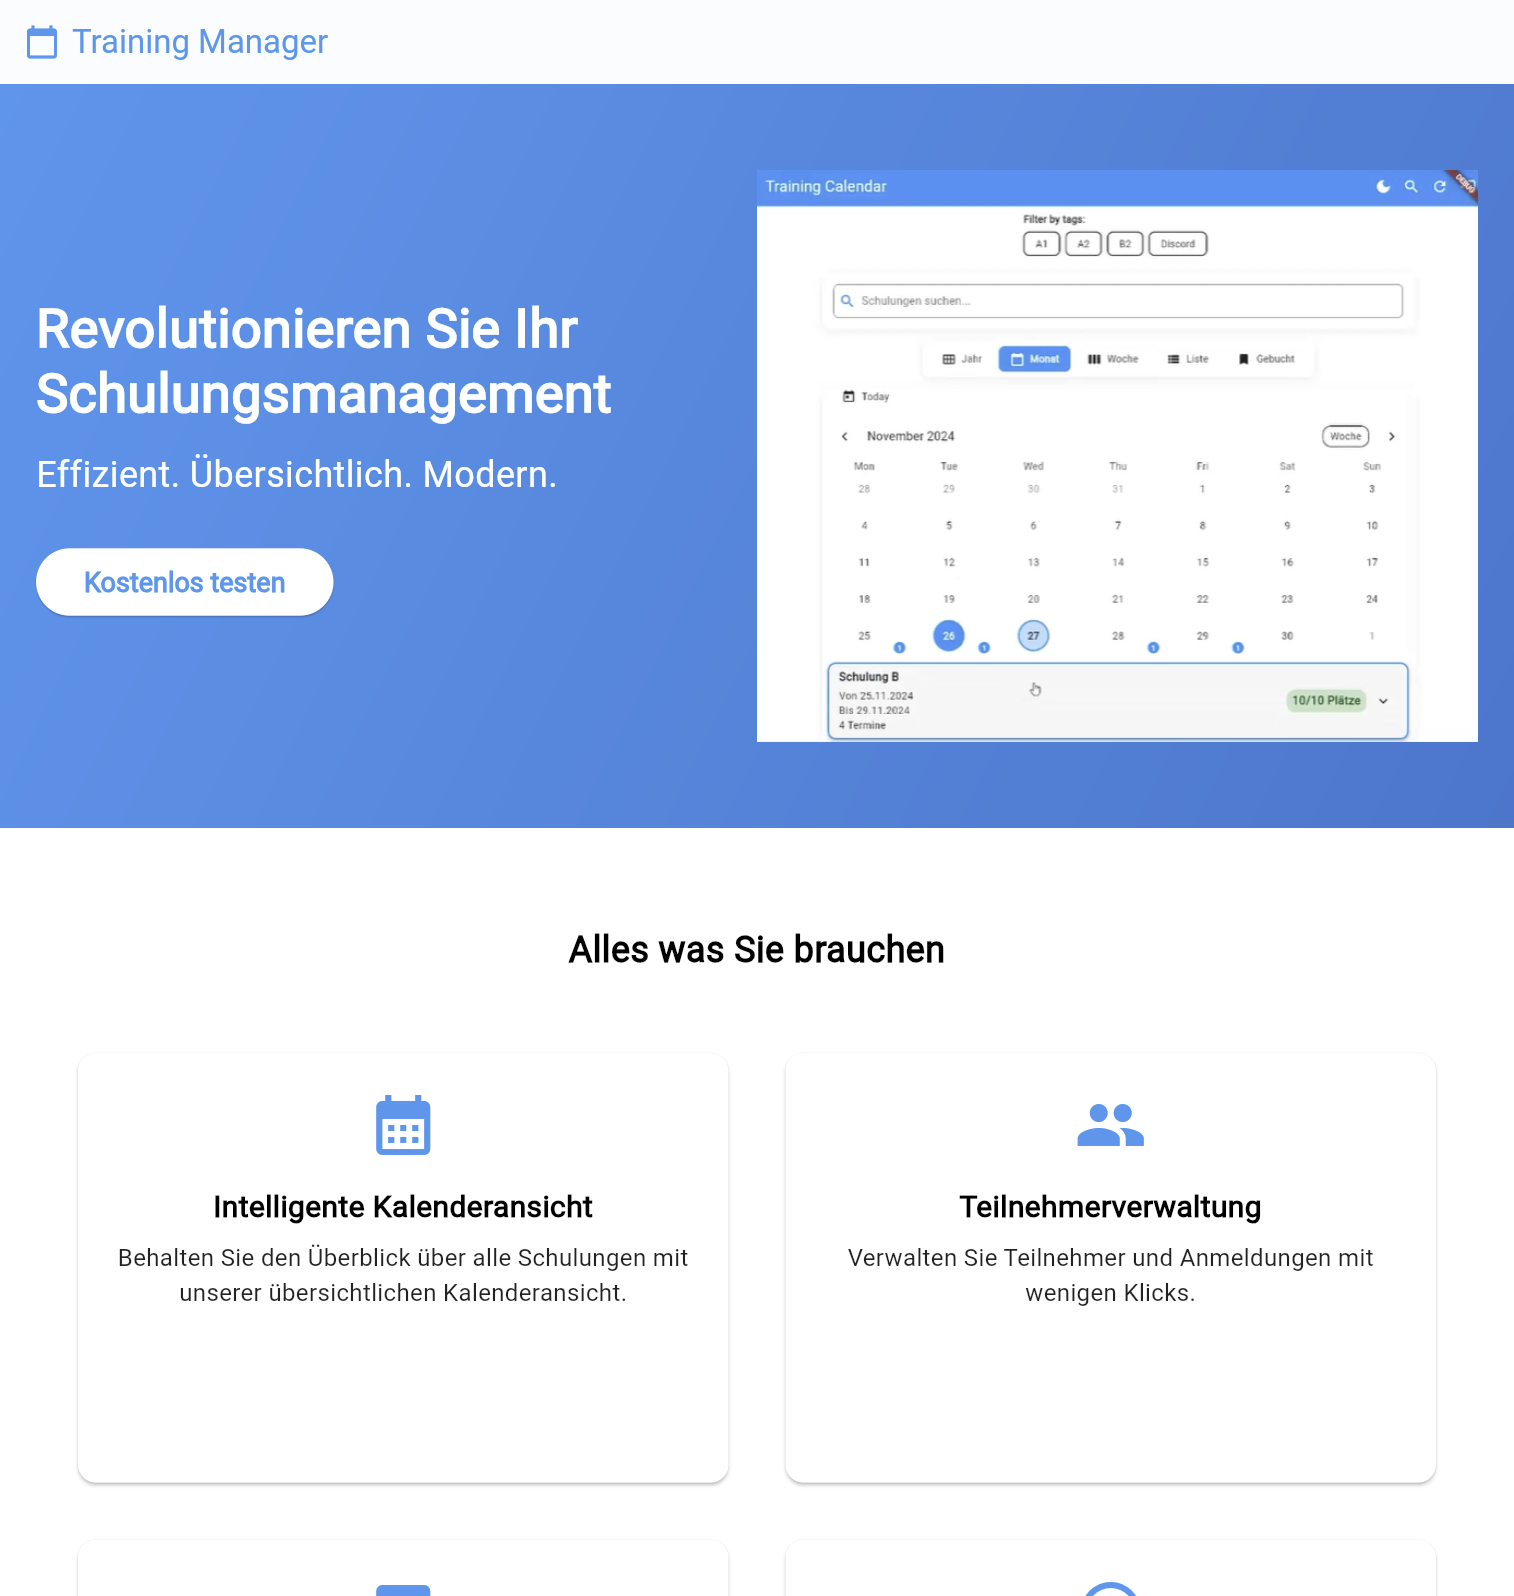
\includegraphics[scale=0.19]{img/flutter_31.png}
        \caption{Startseite}
        \label{HomeBE}
    \end{figure}
\section{Optionen Darstellung}

Im Kalender wurden mehrere Optionen implementiert, die in der Abbildung \ref{OptionenBE} dargestellt sind. Eine dieser Optionen ist
die blaue Leiste, die der Navigation zwischen den einzelnen Fenstern dient und Änderungen des Farbschemas ermöglicht. Über diese
Funktion gelangt man zurück zum Homescreen, öffnet ein Fenster zur Suche, wechselt das Farbschema in den Dark Mode oder kann die
Einstellungen des persönlichen Profils bearbeiten. Sollte der Nutzer noch nicht angemeldet sein, wird diese Leiste als
Login-Fenster angezeigt. \newline

Unterhalb der Navigationsleiste befindet sich eine Funktion, mit der Schulungen nach bestimmten Tags gefiltert werden können. In
diesem Fall wurden als Beispiele die Fachübergreifenden Kompetenzen des CAS gewählt. Bei anderen Schulungen, wie etwa
Sicherheitsunterweisungen, könnte hier auch die dazugehörige ID angezeigt werden. Durch das Anklicken eines Tags wird eine
Filterung nach diesem Kriterium vorgenommen. \newline

Unter der Tag-Filterung ist eine Freitextsuche implementiert, die es ermöglicht, durch alle relevanten Informationen eines 
Trainings zu suchen. So kann nach dem Trainingsnamen, dem Startdatum oder auch dem Namen des Trainers gesucht werden. Sowohl
die Filterung durch die Suche als auch die Tag-Filterung wird bei der Darstellung jeder Kalenderansicht berücksichtigt.\newline

Eine weitere Option ermöglicht es, die Schulungen in verschiedenen Zeiträumen anzuzeigen. Der Nutzer kann zwischen den Ansichten 
„Jahr“, „Monat“ und „Woche“ wählen, wobei die Monatsansicht die Standarddarstellung darstellt. Neben der Darstellung im Kalender
kann die Schulungsliste auch in Listenform angezeigt werden. In dieser Ansicht kann der Nutzer zwischen einer Filterung nach allen
Schulungen oder nur nach den gebuchten Schulungen wählen.\newline

  \begin{figure}[htbp!]
    \centering
    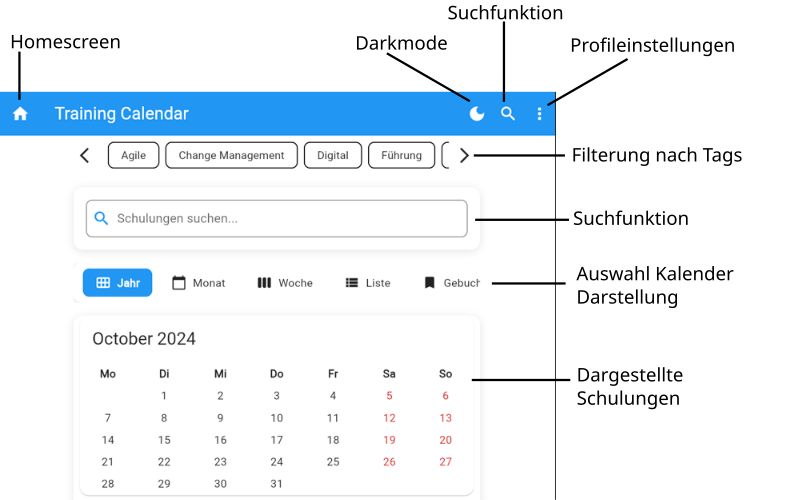
\includegraphics[scale=0.7]{img/Flutter_Optionen.png}
    \caption{Option in der Kalenderansicht}
    \label{OptionenBE}
\end{figure}

\subsection{Kalenderansicht}
In der Kalenderansicht werden Tage, an denen Trainings angeboten werden, mit orangen und blauen Punkten markiert. Ein orangefarbener
Punkt bedeutet, dass es sich um eine mehrtägige Schulung handelt, während ein blauer Punkt darauf hinweist, dass die Schulung nur
an einem Tag stattfindet. In der Monats- und Wochenansicht sind zusätzlich Nummern in diesen Punkten enthalten, die angeben, wie
viele Schulungen an diesem Tag angeboten werden. Dieses unterschiedliche Verhalten ist in der Abbildung \ref{MarkierungSchulung}
dargestellt. Es ist ersichtlich, dass in der Jahresansicht am 24. Dezember nur zwei Punkte angezeigt werden, während in der 
Monatsansicht zusätzlich Zahlen zu sehen sind, die die Anzahl der Schulungen an diesem Tag angeben.
Ist eine Schulung an einem Tag gebucht, wird dieser Tag zusätzlich rot umrandet.

\begin{figure}[htbp!]
    \centering
    \begin{subfigure}[b]{0.45\textwidth}
        \centering
        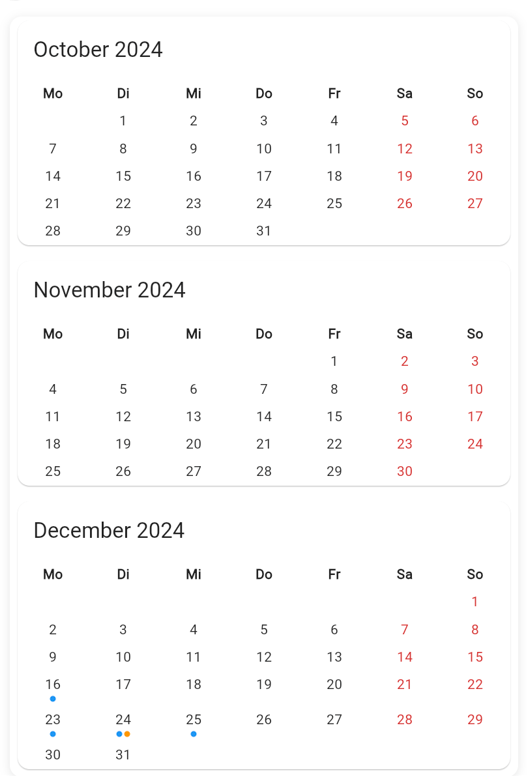
\includegraphics[scale=0.6]{img/Markierung_Dezember_JAhresansicht.png}
        \caption{Jahresansicht}
    \end{subfigure}
    \hfill
    \begin{subfigure}[b]{0.45\textwidth}
        \centering
        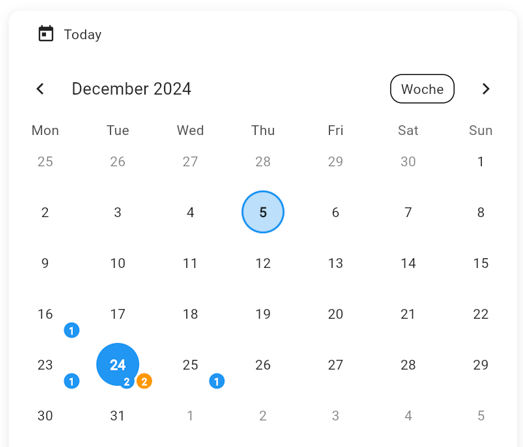
\includegraphics[scale=0.6]{img/Markierung_Dezember_Monatansicht.png}
        \caption{Monatsansicht}
    \end{subfigure}
    \caption{Darstellung der unterschiedlichen Markierungen der verfügbaren Schulungen}
    \label{MarkierungSchulung}
\end{figure}


\subsection{Schulungsinformationen}
Um genauere Informationen zu erhalten, muss der Tag im Kalender angeklickt werden. Anschließend erscheint die Ansicht, die
in Abbildung \ref{InformationenBE} dargestellt ist. Durch Scrollen kann man alle Schulungen durchsehen. Zudem erhält man durch
das Anklicken einer Schulung weitere Informationen, wie beispielsweise die Kontaktdaten des Dozenten, eine Beschreibung der
Schulung sowie die Startzeiten.

\begin{figure}[htbp!]
    \centering
    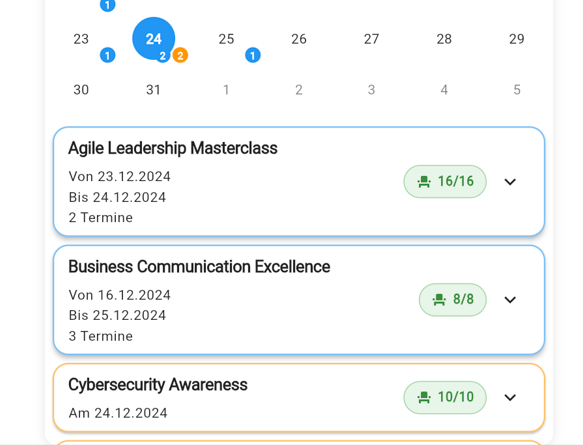
\includegraphics[scale=0.7]{img/trainingsinformationen.png}
    \caption{Informationen zu den Trainings}
    \label{InformationenBE}
\end{figure}

Entscheidet man sich, ein Training zu buchen, so kann man einen Haken setzen, um eine Buchungsbestätigung zu erhalten. 
Dadurch wird dem Benutzer eine E-Mail als Buchungsbestätigung zugesendet.

\subsection{Anbieteransicht}
Meldet man sich als Anbieter von Schulungen in der App an, so hat man die Möglichkeit, Trainings zu erstellen und diese zu 
bearbeiten. In Abbildung \ref{AnbieterBE} sind die verschiedenen Beschreibungsmöglichkeiten für eine Schulung dargestellt.
Die Auswahl des Datums kann dabei in einer Kalenderansicht erfolgen, in der der gesamte Zeitraum markiert wird, in dem die
Schulung stattfindet.

\begin{figure}[htbp!]
    \centering
    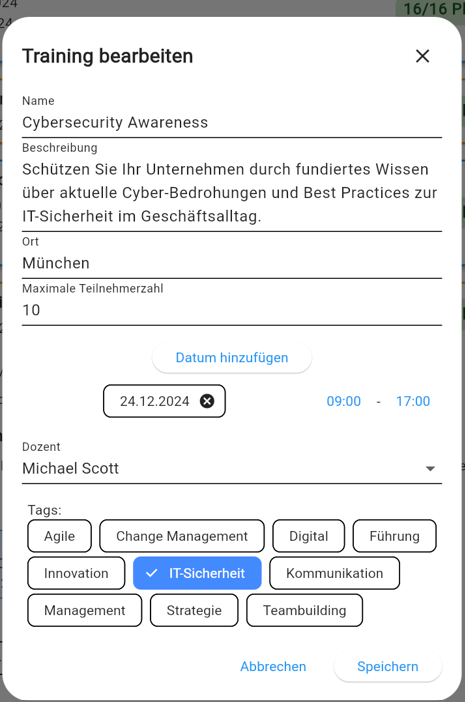
\includegraphics[scale=0.7]{img/BearbeitungAnbierteransicht.png}
    \caption{Bearbeiteransicht}
    \label{AnbieterBE}
\end{figure}

